This section defines transactions and their relationship to each other and to
external data. It also defines a (de-)serialization format to and
from the binary format that is transferred over the wire. In Figure
\ref{fig:transactions} a chain of transactions, with relevant fields, is
shown. This example includes three hosts that have cloned the page and in total
three updates.

\begin{figure}[htp]
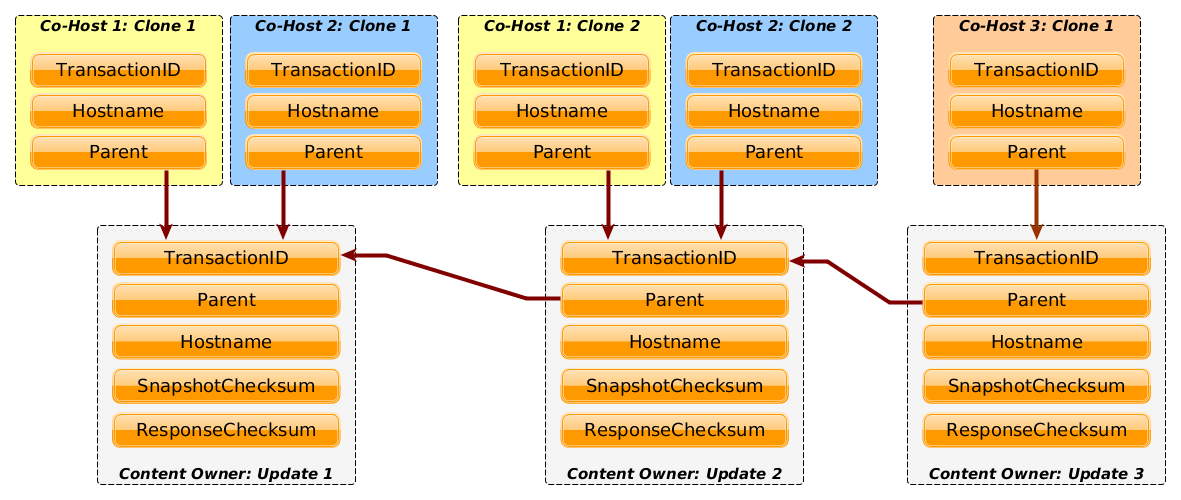
\includegraphics[width=\textwidth]{transactions.png}
\label{fig:transactions}
\caption{Transaction chain example for one page.}
\end{figure}

\subsection{UPDATE Transaction Definition}

Update transactions can only be created by the page creator. Additional to the
proof of ownership they also include a reference to the new content, with
related checksums.

\begin{table}[ht]
  \centering
  \begin{tabular}{|g|p{10cm}|}
    \hline
    \multicolumn{2}{|c|}{\textbf{TRANSACTION HEADER}}\\
    \hline
    \textbf{TransactionID} & Double SHA256 hash of this transaction.\\
    \hline
    \textbf{Parent} & The previous update \textit{TransactionID}\\
    \hline
    \textbf{ScriptSig} & \textbf{TODO Future Work:} Proof here ownernship of
    the hostname and all requirements that come with this update.\\
    \hline
    \textbf{Hostname} & The tor hidden service onion hostname of this page.
    Tor hidden services are needed to be able to host page behind firewalls
    and NATs. Additional they protect the identity of the content owner and
    more importantly of clone hosts.\\
    \hline
    \multicolumn{2}{|c|}{\textbf{CONTENT SECTION}}\\
    \hline
    \textbf{Snapshot} & The hash value of the content. This hash value is used
    to find all peers in the Distributed Hash Table (DHT) that share currently
    this snapshot. The DHT is bootstrapped by using all active hostname in the
    blockchain. For increased compatibility the MAGNET URI scheme is used.\\
    \hline
    \textbf{SnapshotChecksum} & Checksum of the Snapshot content, used to
    verify if the downloaded data.\\
    \hline
    \textbf{ResponseChecksum} & Checksums for all endpoints of this page.
    Makes each page verifiable and hence could be served by a random node. If
    the returned content does not match the here checksum the response is
    invalid.\\
    \hline
    \textbf{Flags} & \textbf{TODO Future Work:} Could be used for
    differentiation between incremental and full updates, but also indicating
    that this page is not hosted anymore and could be deleted.\\
    \hline
  \end{tabular}
\end{table}

\subsection{CLONE Transaction Definition}

Clone transactions are created and propagated by all hosts that start hosting
a page or if they receive a new update transaction. This transactions always
link back to exactly one update transaction.

\begin{table}[ht]
  \centering
  \begin{tabular}{|g|p{10cm}|}
    \hline
    \textbf{TransactionID} & Double SHA256 hash of this transaction.\\
    \hline
    \textbf{Parent} & The previous update \textit{TransactionID}\\
    \hline
    \textbf{ScriptSig} & \textbf{TODO Future Work:} Proof here ownernship of
    the hostname and all requirements that come with this update.\\
    \hline
    \textbf{Hostname} & The tor hidden service onion hostname of this page.
    Tor hidden services are needed to be able to host page behind firewalls
    and NATs. Additional they protect the identity of the content owner and
    more importantly of clone hosts.\\
    \hline
    \textbf{Flags} & Possible values are: \textit{CLONE} when new update was
    received or \textit{PURGE} if the page is not hosted anymore.\\
    \hline
  \end{tabular}
\end{table}
